%% For double-blind review submission, w/o CCS and ACM Reference (max submission space)
\documentclass[acmsmall,anonymous,review]{acmart}\settopmatter{printfolios=true,printccs=false,printacmref=false}
%% For double-blind review submission, w/ CCS and ACM Reference
%\documentclass[sigplan,10pt,review,anonymous]{acmart}\settopmatter{printfolios=true}
%% For single-blind review submission, w/o CCS and ACM Reference (max submission space)
%\documentclass[sigplan,10pt,review]{acmart}\settopmatter{printfolios=true,printccs=false,printacmref=false}
%% For single-blind review submission, w/ CCS and ACM Reference
%\documentclass[sigplan,10pt,review]{acmart}\settopmatter{printfolios=true}
%% For final camera-ready submission, w/ required CCS and ACM Reference
%\documentclass[sigplan,10pt]{acmart}\settopmatter{}

%% Conference information
%% Supplied to authors by publisher for camera-ready submission;
%% use defaults for review submission.
\acmConference[PL'18]{ACM SIGPLAN Conference on Programming Languages}{January 01--03, 2018}{New York, NY, USA}
\acmYear{2018}
\acmISBN{} % \acmISBN{978-x-xxxx-xxxx-x/YY/MM}
\acmDOI{} % \acmDOI{10.1145/nnnnnnn.nnnnnnn}
\startPage{1}

%% Copyright information
%% Supplied to authors (based on authors' rights management selection;
%% see authors.acm.org) by publisher for camera-ready submission;
%% use 'none' for review submission.
\setcopyright{none}
%\setcopyright{acmcopyright}
%\setcopyright{acmlicensed}
%\setcopyright{rightsretained}
%\copyrightyear{2017}           %% If different from \acmYear

%% Bibliography style
\bibliographystyle{ACM-Reference-Format}
%% Citation style
%\citestyle{acmauthoryear}  %% For author/year citations
%\citestyle{acmnumeric}     %% For numeric citations
%\setcitestyle{nosort}      %% With 'acmnumeric', to disable automatic
                            %% sorting of references within a single citation;
                            %% e.g., \cite{Smith99,Carpenter05,Baker12}
                            %% rendered as [14,5,2] rather than [2,5,14].
%\setcitesyle{nocompress}   %% With 'acmnumeric', to disable automatic
                            %% compression of sequential references within a
                            %% single citation;
                            %% e.g., \cite{Baker12,Baker14,Baker16}
                            %% rendered as [2,3,4] rather than [2-4].


\usepackage{graphicx}
\usepackage{subfig}
\usepackage{caption}
%\usepackage{subcaption}
\usepackage[export]{adjustbox}

\begin{document}

% \newcommand{\charcoal}{Charcoal}
\newcommand{\charcoal}{DblBlind}
\newcommand{\atomic}{\texttt{atomic}}
\newcommand{\asyncs}{async$*$}

\special{papersize=8.5in,11in}
\setlength{\pdfpageheight}{\paperheight}
\setlength{\pdfpagewidth}{\paperwidth}

% \titlebanner{Preprint.  Please do not redistribute}        % These are ignored unless
% \preprintfooter{Preprint.  Please do not redistribute}   % 'preprint' option specified.

\title{Atomicity in Cooperative Concurrency: Measurements, Language Design and Implementation}
% \subtitle{\ldots and How to Make Cooperative Concurrency Safer with \texttt{atomic}}

%% Author information
%% Contents and number of authors suppressed with 'anonymous'.
%% Each author should be introduced by \author, followed by
%% \authornote (optional), \orcid (optional), \affiliation, and
%% \email.
%% An author may have multiple affiliations and/or emails; repeat the
%% appropriate command.
%% Many elements are not rendered, but should be provided for metadata
%% extraction tools.

%% Author with single affiliation.
\author{Benjamin Ylvisaker}
% \authornote{with author1 note}          %% \authornote is optional;
                                        %% can be repeated if necessary
% \orcid{nnnn-nnnn-nnnn-nnnn}             %% \orcid is optional
\affiliation{
  \position{Assistant Professor}
  \department{Department of Math and Computer Science}
  \institution{Colorado College}
  \streetaddress{14 E Cache La Poudre St}
  \city{Colorado Springs}
  \state{CO}
  \postcode{80903}
  \country{USA}
}
\email{bylvisaker@coloradocollege.edu}


\begin{abstract}

  ABSTRACT
%% This paper is about combining cooperative concurrency with atomic blocks.
%% In particular, we address two primary questions:
%% Why might this combination be useful?
%% What is tricky about making a clean semantics and implementation for languages that combine these concepts?

%%   The sophistication of multitasking in mainstream software has increased in recent years, thanks to the increasing richness of network communication, physical world interaction and multi-process software architectures.
%% These trends have pushed programming languages to offer better ways of writing such code.
%% As just one example of this trend, in recent years some flavor of coroutine has been standardized (or is heading towards standardization) in JavaScript, Swift, and C++.

%% This paper makes two primary contributions.
%% The first is an empirical study of multitasking in modern web applications.
%% Our primary finding is that in current practice, web JavaScript code tends to exhibit risky patterns, from the perspective of atomicity.
%% We argue that an \texttt{atomic} block primitive should be added to languages to help programmers avoid atomicity bugs.

%% We also experiment with two implementations of cooperative threads plus atomic: a JavaScript library and a dialect of C.
%% This investigation shows that this language design can be implemented in a flexible and efficient way.

\end{abstract}


%% 2012 ACM Computing Classification System (CSS) concepts
%% Generate at 'http://dl.acm.org/ccs/ccs.cfm'.
\begin{CCSXML}
<ccs2012>
<concept>
<concept_id>10011007.10011006.10011008</concept_id>
<concept_desc>Software and its engineering~General programming languages</concept_desc>
<concept_significance>500</concept_significance>
</concept>
<concept>
<concept_id>10003456.10003457.10003521.10003525</concept_id>
<concept_desc>Social and professional topics~History of programming languages</concept_desc>
<concept_significance>300</concept_significance>
</concept>
</ccs2012>
\end{CCSXML}

\ccsdesc[500]{Software and its engineering~General programming languages}
\ccsdesc[300]{Social and professional topics~History of programming languages}
%% End of generated code


%% Keywords
%% comma separated list
%% \keywords are mandatory in final camera-ready submission
\keywords{Cooperative concurrency, Multitasking, Atomicity}

\maketitle

% Outline:
% Introduction
%   Contributions
% Atomic or Interruptible?
%   On Atoms and Interrupts
%   Events
%   Cooperative Threads
%   Coroutines and Async Procedures}
%   What's Wrong with Threads?
% Activities
%   Shared Variables
%   Yield Insertion
%   Atomic
%   System Calls
%   Activities, Compared
% Implementation
%   Call Frame Allocation
%     Contiguous Allocation
%     Individual Heap Allocation
%     Split/Segmented Stacks
%     Dynamic Contiguous Stacks
%     Hot Stacking
%   Yield Implementation
%     Yield in Atomic Mode
%     Function Pointers
%     Yields
%   Asynchronous System Calls
%   Translation
%   Activities in JavaScript
% Evaluation
%   Building an App with Activities
%   Task Memory Overhead
%   Task Spawn and Switching Speed
%   Just Calling
%   Yielding
%   Microbenchmark Summary
% Related Work
%   Other Multitasking Abstractions
% Summary and Discussion



\section{Introduction}

Many applications are highly multitasked.
They have lots of balls in the air at the same time: network communication, queries to databases, multiple I/O modalities to monitor and manage.
Applications use a wide range of features in languages and core libraries to implement this multitasking: threads, event loops, coroutines, async functions, functional reactive programming, etc.\footnotemark{}

\footnotetext{Some of these features are also relevant to \emph{parallelism} (i.e. physical simultaneity), but parallelism is \emph{not} the subject of this paper or the project it describes.}

Many popular application programming frameworks use some form of \emph{cooperative} multitasking, because of the fear that \emph{preemption} too easily causes concurrency bugs.
While the authors of this paper are sympathetic with that fear, we remind the reader that cooperativeness only \emph{reduces} the risk of concurrency defects\footnotemark{}.
There has been much research in the last decade on cataloging, exposing, diagnosing and fixing concurrency bugs in web and mobile applications that use cooperative concurrency.

\footnotetext{This is similar to how garbage collection reduces, but does not eliminate, exposure to memory bugs \cite{Grossman2007}.}

One important concept for avoiding concurrency bugs is \emph{atomicity}.
This idea is nearly universal in the database world, where atomic transactions are used to ensure that multiple reads and writes are performed without interruption.
Herlihy and Moss \cite{Herlihy1993} kicked off decades of research on bringing this idea to general purpose multithreading languages in the form of a code block that can make an arbitrary sequence of statements appear atomic.

% XXX , because of challenges with implementation efficiency and semantic trickines with concurrent access to resources from atomic blocks and non-atomic code

The idea of preemptive multithreading languages with atomic blocks is compelling, but has seen little use outside of research labs because of technical roadblocks.
The broad question addressed in this paper is: Is it a good idea to combine atomic blocks with cooperative concurrency models, like event loops or cooperative threads?
We primarily focus on three sub-questions:
\begin{enumerate}
\item Do atomic blocks bring software engineering benefits to cooperative concurrency?
\item Are there any semantic or language design problems with this combination of features?
\item Are there interesting implementation efficiency issues raised by this combination of features?
\end{enumerate}

We gather evidence for the first question by measuring widely used web applications\footnotemark{}.
We observe that patterns that seem risky from an atomicity perspective are common.
In particular, there are many short-duration chains of continuations.
We believe it would be easy for a developer to test such code and effectively assume atomicity for the chain, even though it is possible for conflicting tasks to execute in gaps between continuations.

\footnotetext{We study web applications for the simple reason that a large amount of presumably highly vetted code is easily available for the studying.}

In investigating the second question, we noticed the following conflict with combining atomic blocks and anonymous cooperative concurrency:
\begin{enumerate}
\item There are multiple reasonable definitions for the nesting of atomic blocks and task spawns; no interpretation works well in all contexts.
\item Many cooperative concurrency frameworks are \emph{anonymous} in the sense that they lack an explicit notion of task identity.
  This makes it hard for the system to know whether the programmer intended an asynchronous continuation to be logically a single interrupted task, or a new concurrent task.
  This further compounds the problem with atomic and spawn nesting, because spawns cannot be identified unambiguously.
\end{enumerate}
To the best of our knowledge, this is a novel observation.
This implies that \emph{if} a cooperative multitasking framework is to include atomic blocks, it should have explicit task identities (i.e. some flavor of cooperative multithreading).

To investigate the third question, we implemented cooperative threads with atomic blocks in two contexts: as a library built on top of JavaScript's coroutines (\texttt{function*}) and \texttt{Promises}, and as a dialect of C.
We observe that such a library can be used with modest code complexity relative to popular JavaScript patterns, and that it mostly integrates well with legacy code.
In the C dialect implementation we discover a new call frame allocation strategy -- enabled by atomic blocks -- that combines the speed benefits of contiguous frame allocation with the memory benefits of individual linked frame allocation.

\begin{figure*}
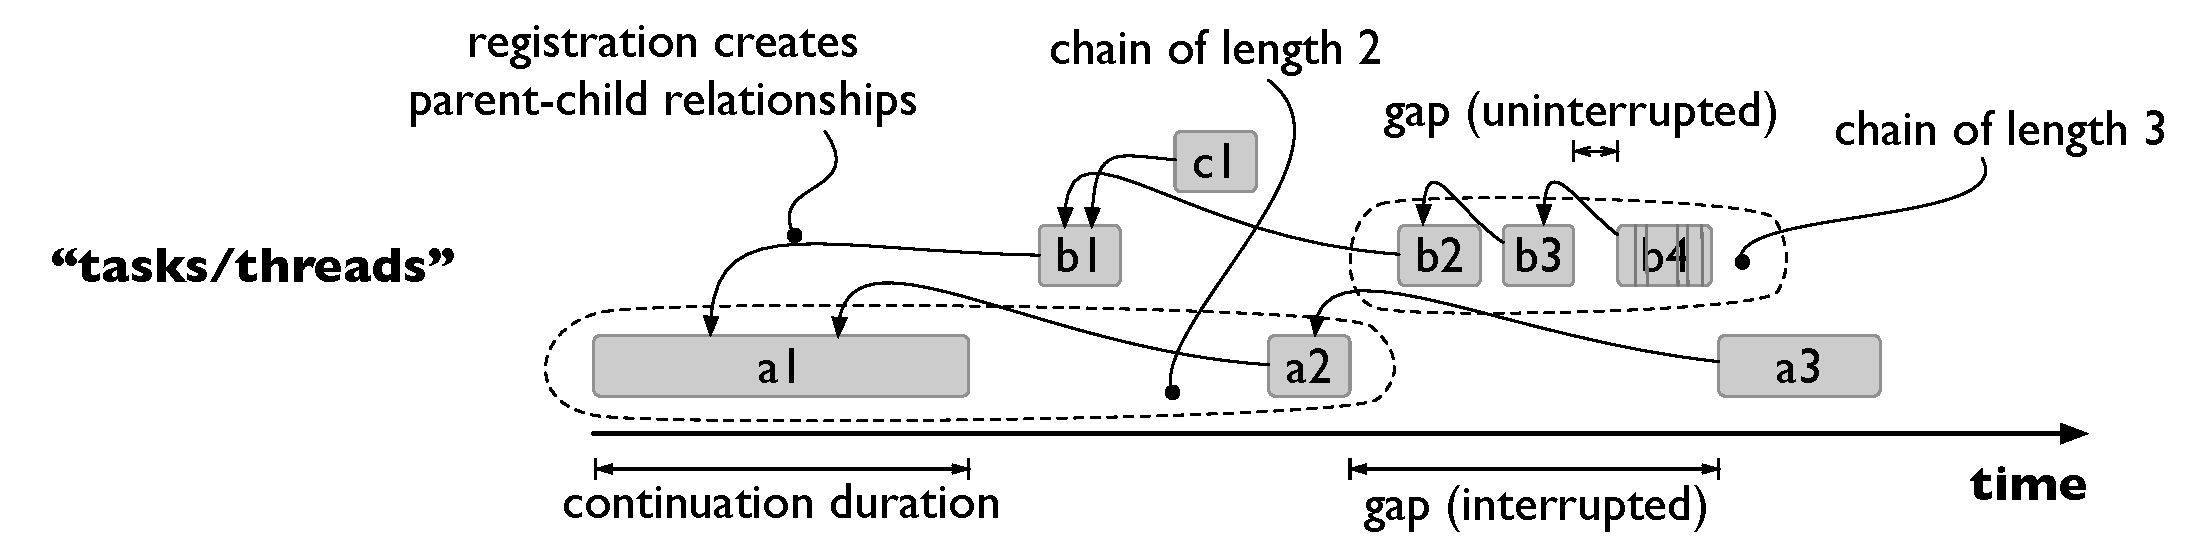
\includegraphics[width=0.9\textwidth]{Figures/continuation_tree}
\caption{The features of JavaScript event execution that our modified Chromium browser measures.
  The gray boxes are continuations.
  The continuations are arranged in rows to suggest that they belong to the same task/thread.
  However, event loop systems do not have this concept, so this is purely an intuitive interpretation.
  For example, a2 and b1 are both children of a1, and there is no way for the system to know what logical task either belongs to.}
\label{fig:continuation_tree}
\end{figure*}

In summary, the contributions of this paper are:
\begin{itemize}
\item A measurement study of multitasking in web applications.
\item An analysis of the conflict between atomic blocks and anonymous multitasking.
\item An exploration of integrating cooperative threading with atomic blocks into an existing multitasking ecosystem.
\item A new call frame allocation strategy for languages with atomic blocks.
\end{itemize}

All code and data described in this paper is available publicly on GitHub [URL removed for blind review].

\section{Multitasking in Web JavaScript}

We begin with a brief (and partial) history of multitasking in JavaScript.
In the beginning, the designers of JavaScript decided that preemptive threads caused an unacceptably high risk of concurrency bugs.
One good entry into the vast literature on the difficulties of diagnosing and fixing multithreading defects is \cite{Lu2008}.
These challenges have long been understood; more than two decades ago Ousterhout wrote a popular critique of threads \cite{Ousterhout1996}.

Early versions of JavaScript supported only event-based concurrency.
The simple picture of the implementation of JavaScript is that there is a single event dispatcher that stores a collection of functions waiting for some enabling condition.
These functions can be registered by primitive APIs, like \texttt{setTimeout}.
In all cases we refer to such registered functions as \emph{continuations}.
We refer to a continuation plus its enabling condition as an \emph{event}.
When an event becomes ready, the dispatcher may execute its continuation.

Simple event programming has some serious drawbacks.
For example, management of resources whose lifetime spans multiple events and propagation of errors can be quite tricky.
This leads to a style of programming referred to as \emph{stack ripping} \cite{Adya2002}, or more colloquially \emph{callback hell}.
These and more subtle problems are well analyzed and criticized by von Behren et al. in \cite{Behren2003a}.

The increasingly sophisticated multitasking in modern applications and the well-known problems with events and threads have increased the use of alternatives in recent years, the most popular of which are \emph{coroutines} and \emph{async procedures}.
Examples include async/await, which was added to C\#/.Net in 2012; function generators (\texttt{function*}, essentially coroutines), which were added to JavaScript with ECMAScript 6 (standard published in 2015); even the staid C++ community is considering adding native support for coroutines (currently on the short list for inclusion in the C++20 standard).
Coroutine implementations are not \emph{new}; for example, Modula-2 had coroutines in the 1980s and several ``scripting'' languages (Ruby, Python, Lua) added support in the early aughts.
However, coroutines and async functions were not widely used in application programming until relatively recently.

The most recent versions of JavaScript have native support for promises, coroutines and async functions.
A style of programming that combines async functions and Promise chaining has become popular in JavaScript communities.
This style of programming makes multitasking much more convenient than programming with explicit callbacks.
This evolution in style has made it feasible for more developers to write more highly multitasked applications.

The theme of the measurements in the remainder of this section is: perhaps there are ways in which it is now too easy to write highly asynchronous code.
In particular, the safety of JavaScript and similar languages has always relied heavily on the atomicity of relatively long-running (in the microscopic computer clock rate sense) functions.
As programmers chop applications up into chains of smaller functions, atomicity problems reemerge as an interesting risk.
We do not show any specific atomicity violations in this paper.
Rather, the measurements demonstrate that all the empirical preconditions for atomicity violations are quite common.

\subsection{Measurements}

We modified a version of Chromium to gather data on JavaScript behavior from web applications.
Figure \ref{fig:continuation_tree} illustrates the features of JavaScript execution that our modified browser measures:

\begin{itemize}
\item Continuation duration is the time difference between when the dispatcher passes control to a continuation and when it returns.
\item We measure both the duration and number of microtasks in microtask batches.
  More on microtasks below.
  (The vertical lines in continuation b4 in the Figure are meant to suggest individual microtasks within a batch.)
\item Parent-child relationships are inferred by recording which continuation (the parent) is running when potential children are registered; this relation is referred to as \emph{async-contexts} in \cite{Loring2017}.
  There is actually a more subtle distinction between what that paper refers to as \emph{linking contexts} and \emph{causal contexts} when dealing with Promises.
  We will primarily be analyzing raw callbacks, for which this distinction does not exist.
\item A \emph{gap} is the time difference between the start of a continuation and the end of its parent.
  A gap is \emph{interrupted} if \emph{any} other continuation runs between parent and child.
\item Figure \ref{fig:continuation_tree} suggests with the horizontal rows an intuitive notion of tasks, where a registered continuation can either be a logical continuation of its parent's task or a newly spawned concurrent task.
  This concept is sufficiently important that several libraries and tools have related ideas, like Zones in AngularJS, Async Hooks in Node.js and Async Call Stacks in the Chrome Developer Tools.
  Unfortunately, it is not part of standard JavaScript, so in general it is not possible to automatically and precisely infer.
\end{itemize}

% Async Hooks. 2016. https://github.com/nodejs/diagnostics/tree/ master/tracing/AsyncWrap.
% Async Call Stacks. 2014. http://www.html5rocks.com/en/tutorials/developertools/async-call-stack/.
% [26] Zones. 2014. https://github.com/angular/zone.js.

\begin{figure}
    \centering
    \begin{minipage}[t]{0.47\textwidth}
        \centering
        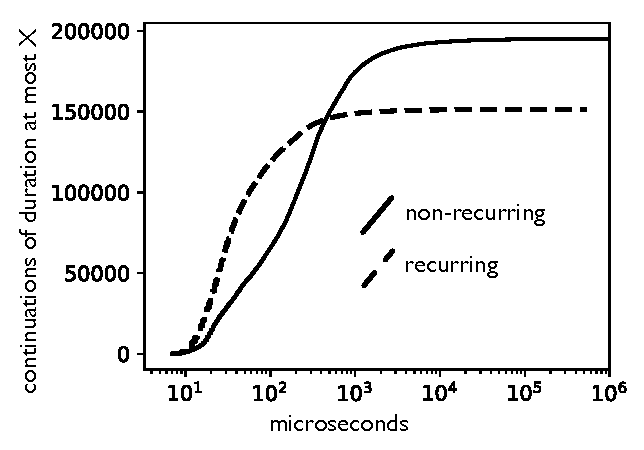
\includegraphics[width=1.0\textwidth]{Graphs/durations_bw}
        \caption{Most continuations are short.
  Many are very short.}
        \label{fig:graph_duration}
    \end{minipage}\hfill
    \begin{minipage}[t]{0.47\textwidth}
        \centering
        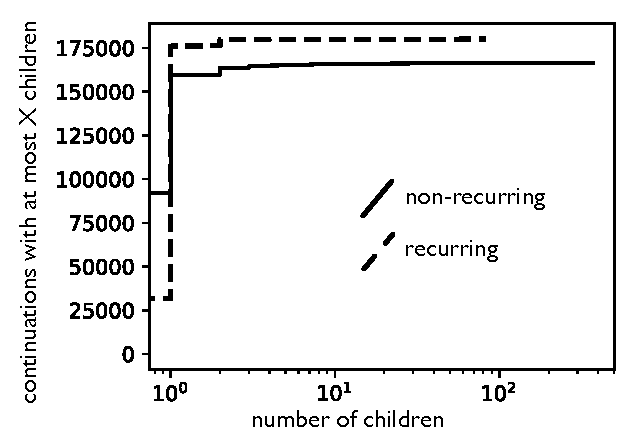
\includegraphics[width=1.0\textwidth]{Graphs/branching_bw}
        \caption{Most continuations have one child.
A few have many, many children.}
        \label{fig:graph_branching}
    \end{minipage}
\end{figure}

\subsubsection{Duration}

Our first observation from Figure \ref{fig:graph_duration} is that most continuations are quite short.
A large majority take less than one millisecond, and many are much shorter.
(This figure combines the data for both microtask batches and normal tasks.)

Short continuations are the first precondition for atomicity violations.
If most continuations were long, we would expect it to be less common for a programmer to ``miss'' a gap between them.
Also, it is interesting to see that JavaScript programmers seem to overwhelmingly abide by the norm that function executions should complete quickly, in order to keep applications responsive.
This observation will be important when we discuss API design later.

The difference between the solid and dashed lines in Figure \ref{fig:graph_duration} highlights the importance of recurring events.
In JavaScript, certain APIs, like \texttt{setInterval} and \texttt{XMLHttpRequest} register continuations that the event dispatcher can call multiple times.
As you can see, these recurring continuations account for a majority of the shortest.
(A majority of those are accounted for by status updates on downloading files.)
However, even among the non-recurring continuations, there are still quite a few towards the short end of the distribution.
In several of the measurements and analyses below we \emph{filter out the recurring events}, because they are less relevant to our focus on chains of continuations that could be mistaken for being atomic.

\subsubsection{Branching and Concurrency}

Next, notice in Figure \ref{fig:graph_branching} that most continuations have \emph{at most} one child.
Among recurring continuations there are more with one child; among non-recurring continuations there are more with zero.
The fact that there are many single-child continuations suggests that JavaScript programmers are breaking linear sequences of logic up into multiple continuations.
Presumably they are doing this either intentionally to improve responsiveness, or because of libraries that only offer an async interface.
Otherwise, why not combine these continuations into a single function?

Though most continuations have few children, a few continuations have many.
This can be seen in the long tail in Figure \ref{fig:graph_branching}.
(There are at least a few continuations with hundreds of children!)
A consequence of this branching is that the continuation trees we studied exhibit quite a lot of concurrency.
For each continuation we define its degree of concurrency to be the number of continuations that \emph{will} run \emph{after} it, but were registered before it started.
In other words, how many parent-child edges are ``live'' across each continuation?

Figure \ref{fig:graph_concurrency} shows the results of our concurrency measurements.
Notice that most continuations are concurrent with at least 10 edges, and a substantial minority are concurrent with at least 100.
Again, the high degree of concurrency is \emph{not} direct evidence of atomicity problems, but it is another precondition.
If most continuations had a low degree of concurrency there would be little opportunity for a conflicting task to create an atomicity violation.

\begin{figure}
    \centering
    \begin{minipage}[t]{0.47\textwidth}
        \centering
        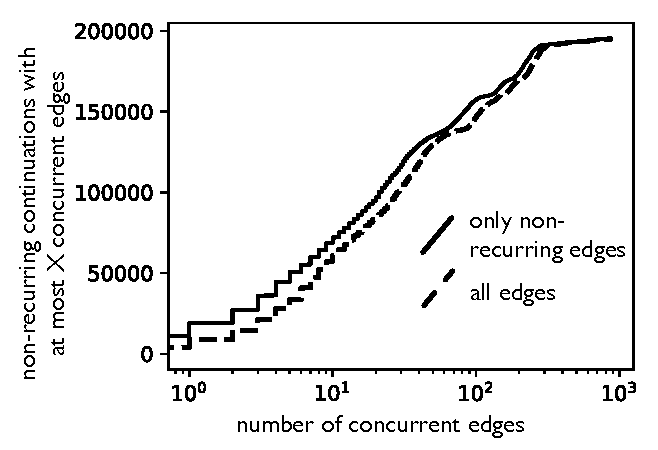
\includegraphics[width=1.0\textwidth]{Graphs/concurrency_bw}
        \caption{Most continuations are concurrent with several parent-child edges.
        In this graph we only include non-recurring continuations.}
        \label{fig:graph_concurrency}
    \end{minipage}\hfill
    \begin{minipage}[t]{0.47\textwidth}
        \centering
        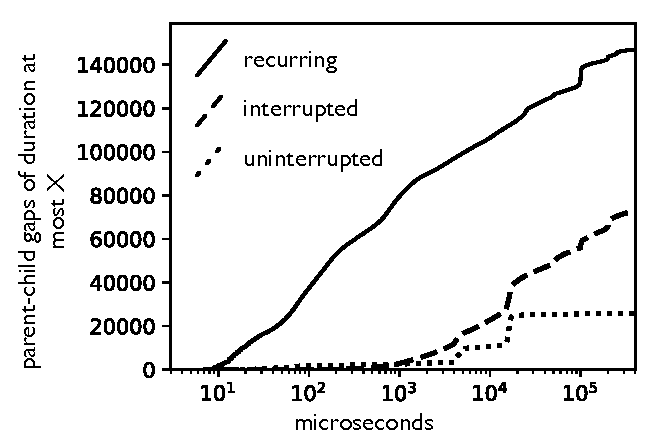
\includegraphics[width=1.0\textwidth]{Graphs/gaps_bw}
        \caption{Most gaps are of reasonable length, but a nontrivial percentage are quite short (under one millisecond, or even 100 microseconds).
  This graph is truncated at half a second, because we are not interested in long gaps.
  There is only a small number of longer gaps.}
        \label{fig:graph_gaps}
    \end{minipage}
\end{figure}

\subsubsection{Gaps and Chains}

The last basic measurements of continuation trees that we consider are the lengths of parent-child gaps and short chains.
Figure \ref{fig:graph_gaps} shows that many gaps are quite short.
The majority of the shortest gaps are between recurring events, which are less interesting to us.
However, there are still quite a few gaps between non-recurring events that are below 10 milliseconds.

A particularly interesting feature to notice is that there are thousands of uninterrupted gaps in the 100s of microseconds range, but far fewer interrupted gaps.
This means that interruption of gaps of that size is possible, but rare.

Figure \ref{fig:graph_chains} shows the duration of continuation chains of length 2, 3 and 4 (that is, the time difference between the beginning of first continuation in the chain and the end of the last).
For this graph we filtered out all chains with recurring continuations.
This data is not surprising based on the continuation duration and gap data and presented above.
We see that while many chains are of a fairly reasonable duration (say, dozens to hundreds of milliseconds), there is a non-trivial fraction under 10 milliseconds, and even some under 1 millisecond.

Yet again, short gaps and short duration chains are \emph{not} direct evidence of atomicity problems.
However, it is easy to imagine a rigorous testing regime that never observed an execution where one of these short gaps was interrupted.

\begin{figure}
    \centering
    \begin{minipage}[t]{0.47\textwidth}
        \centering
        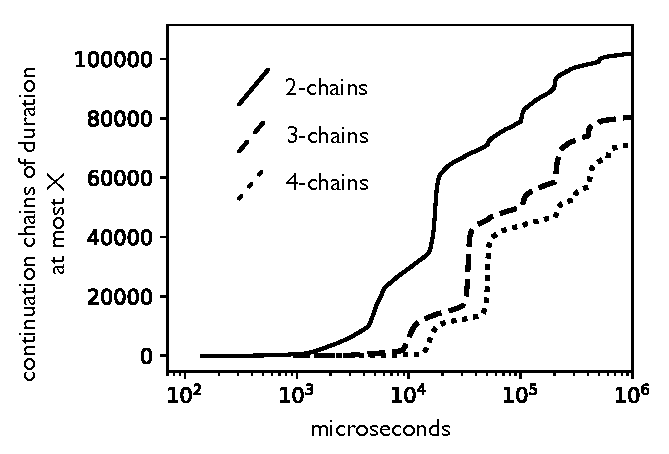
\includegraphics[width=1.0\textwidth]{Graphs/chains_bw}
        \caption{XXX chains.}
        \label{fig:graph_chains}
    \end{minipage}\hfill
    \begin{minipage}[t]{0.47\textwidth}
        \centering
        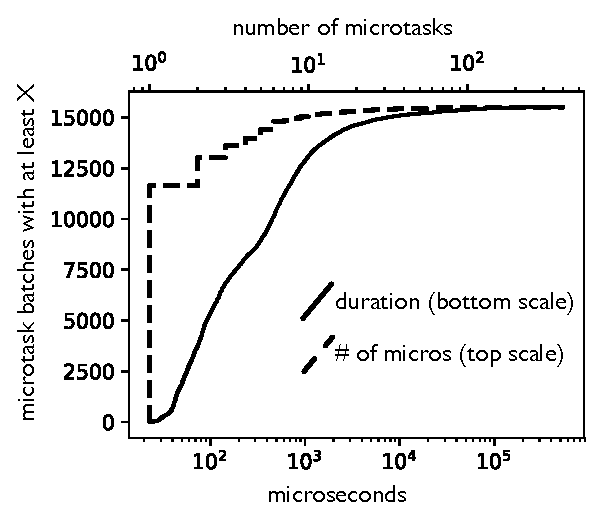
\includegraphics[width=1.0\textwidth]{micros_graph_bw}
        \caption{Most microtask batches are short, but a nontrivial number are long enough to possibly exceed the time and/or microtask count limits of some reasonable implementations.}
        \label{fig:graph_microtasks}
    \end{minipage}
\end{figure}

\subsubsection{Microtasks}

In this subsection, we look at microtasks, which are tangential to the main plot of this paper, but still somewhat interesting.
Microtasks are a special subset of events in JavaScript; the most common source of microtasks is Promise resolution.
Unlike regular events, as soon as at least one microtask is registered, the interpreter switches to running microtasks.
During the execution of a microtask, more microtasks can be registered, and the interpreter will not run another continuation from the normal event dispatcher until the microtask queue is empty.

Figure \ref{fig:graph_microtasks} shows information about the durations and microtask counts of microtask batches.
Most batches are fairly short/small by both metrics, which is good from a concurrency bug perspective.
However, a nontrivial minority of microtask batches get into the 10s and even 100s of milliseconds and/or dozens or hundred of microtasks.
At that size, these microtask batches start to be potential responsiveness problems.
When batches of microtasks get too long, programmers may make ad hoc decisions about where to break them up, thus potentially creating more opportunities for atomicity problems.

\subsubsection{Atomic Can Cause Unresponsiveness}

One interesting metric that we were \emph{not} able to derive from our continuation trees is the variance in durations of dynamic instances of specific source-level chains of continuations.
This is an interesting metric because it is evidence for how likely it is that using a source-level atomic block would increase the risk of unresponsiveness.
To be concrete, imagine a block of source code that generates a chain of continuations that is usually very short, but is occasionally long.
If such a block of source was wrapped in atomic it could create a responsiveness problem in those occasional situations.
The reason this metric is hard to measure on popular websites is that most of them seem to deploy JavaScript code that has been compiled (e.g. by Babel or Google Closure) and uses extensive frameworks (like Angular or Relay).
One of the consequences of this is that often there are shim functions around event registration and/or dispatching, which makes it hard to infer source-level information from dynamic traces.

\subsection{Instrumentation and Data Source Details}

TODO

\subsection{Is This Actually a Problem?}

In this paper we do not present any specific atomicity violations, only evidence that risky patterns are common.
This leads us to a couple important questions:
How confident can we be that the patterns we study are associated with real atomicity defects, and are thus worth doing something about?
If these patterns are a valid concern (of any magnitude), what explains their existence in the most widely used web applications?
We will address the second question first.

\subsubsection{An Explanation for the Rise of Short Chains}

There is always a dilemma in cooperative concurrency associated with the durations of whatever the atomic chunks are.
The longer the chunks, the higher the risk of unresponsiveness or at least appearing jittery and potentially missing I/O deadlines.
The shorter the chunks, the higher the risk of splitting some logic that should be atomic into multiple chunks.

This dilemma is particularly acute for library authors, because they bear the responsibility to make their code work well in multiple specific contexts; quite often those contexts are unknown to the library authors.
To be more concrete, when library authors design APIs, they face the choice between making a call atomic or async in some way (callback, Promise, async method, whatever).
In some cases this choice is easy.
If the function always completes quickly, then it should be atomic.
If the function usually takes a long time, then it should be async.

Unfortunately, many functions fall in the awkward middle territory, where some calls are quick and others are not.
For these functions, async is in some sense the easier choice, because long-running atomic calls create immediately obvious responsiveness problems that cannot be easily worked around by applications.
On the other hand, atomicity problems are not as obvious and in principle can be worked around by application-level synchronization.

A similar line of reasoning led the developer's of Microsoft Windows' core Windows Runtime (WinRT) library to replace many atomic procedures with asynchronous ones in Windows 8.
In a post on the Microsoft Developer Blog \cite{Windows8Team2012}, the team explains that they did this for procedures that ``could likely take longer than 50 milliseconds to execute''.

In some recently defined JavaScript APIs, even some functions that will execute quickly in most reasonable contexts have an async interface.
As one example among many, the PBKDF2 key derivation function in the WebCrypto library returns a Promise.
PBKDF2 is a function that takes a number of iterations as a parameter.
On a modern computer the PBKDF2 function takes in the rough neighborhood of one microsecond per iteration.
So the iteration parameter must be set very high for this function to represent a responsiveness problem.
In contexts where the iteration count is lower, the caller would almost certainly prefer an atomic interface.

Consider a more extreme example: sending a network request.
Sending a message over a wide area network will inevitably be slow, and network operations are generally defined to be asynchronous to accommodate this.
However, in a microservices software architecture, applications use network protocols to communicate with other processes that might be running on the same computer.
Depending on the details of a specific request to a peer process, it may actually be fast enough that the requester would prefer to block while waiting for the response.

It is now common practice to use a large number of libraries and frameworks in JavaScript applciation development.
One remarkable metric of this part of the JS ecosystem is that the NPM package repository had over 600,000 modules, as of March, 2018 \cite{ModuleCounts}.

These examples illustrate what we claim is a general trend towards applications using a complex collection of libraries with async interfaces.
The data presented in the previous section is consistent with this now being common practice.

% SPAs, end-to-end encryption

\subsubsection{The Atomicity Violation Struggle is Real}

There has been a great deal of research on atomicity violations in general (e.g., \cite{Lu2008}).
More directly relevant to this paper, several researchers have worked on detecting and classifying concurrency bugs in event-driven web and mobile applications: \cite{Petrov2012, Hsiao2014, Mutlu2015, Zhang2017}.
These papers focus on ``races'', which are related to atomicity violations.
Every atomicity violation involves a race, in some sense, but not every race is part of an atomicity violation.

% Petrov2012  Race Detection for Web Applications
% Hsiao2014  Race Detection for Event-driven Mobile Applications
% Mutlu2015  Detecting JavaScript Races That Matter
% Zhang2017  RClassify: Classifying Race Conditions in Web Applications via Deterministic Replay
% XXX Shin Hong, Yongbae Park, and Moonzoo Kim. Detecting concurrency errors in client-side java script web applications. In IEEE International Conference on Software Testing, Verification and Validation, pages 61– 70, 2014.

Another kind of evidence is analysis of concurrency bugs in JavaScript applications based on real bug databases: \cite{Davis2017, Hong2014, Wang2017}.
The authors of \cite{Davis2017} reported that 69\% of the 16 concurrency bugs they studied involved an atomicity violation, while the authors of \cite{Wang2017} reported 65\% of 57 bugs.
The latter paper goes on to report that of the atomicity violation bugs, 27\% were fixed by adding synchronization or switching to an atomic API.
These papers specifically looked at applications based on Node.js, which is somewhat different from browser JavaScript.
However, with the rising popularity of tools like Webpack, Browserify and Gulp, libraries from the expansive NPM ecosystem are increasingly being used in code written for browsers.
This means that the differences between browser JavaScript and Node.js JavaScript are shrinking.
Also while Node.js has traditionally been used to develop backend servers, it is increasingly being used in client applications via tools like Electron, Cordova and Ionic.

% Davis2017 11/16 atomicity violations
% Wang2017  65% atomicity violations --> 27% fixed by adding synchronization or switching to an atomic API

\subsubsection{Potential Solutions}

The remainder of this paper explores atomic blocks as a mitigation strategy for atomicity problems.
However, we do want to acknowledge that there are other strategies that programmers are surely already using to some extent.

One strategy is to use a ``functional'' style of programming, with immutable data structures and application-level atomic transactions.
If this strategy is used consistently, then it is unimportant how small the atomic chunks are; the likelihood of concurrency bugs depends very little on fine-grained scheduling.

Even if a project is written in the more common imperative style with fine-grained actions with observable effects, careful software engineering can still protect against atomicity violations.
For example, programmers could use an adversarial scheduler during testing to flush out concurrency bugs.

While the authors of this paper have no quibbles with either of these software engineering strategies, we observe that quite a few applications are written with a modest level of software engineering care.
It would be nice if there was a relatively simple tool (like an atomic block) that could help avoid at least some subset of concurrency issues.
Also one note of caution to keep in mind is that some techniques are appropriate for maintaining atomicity within the bounds of a single process, but are less relevant when I/O is involved.

\section{The Tension Between Anonymous Multitasking and Atomic}

\begin{figure}
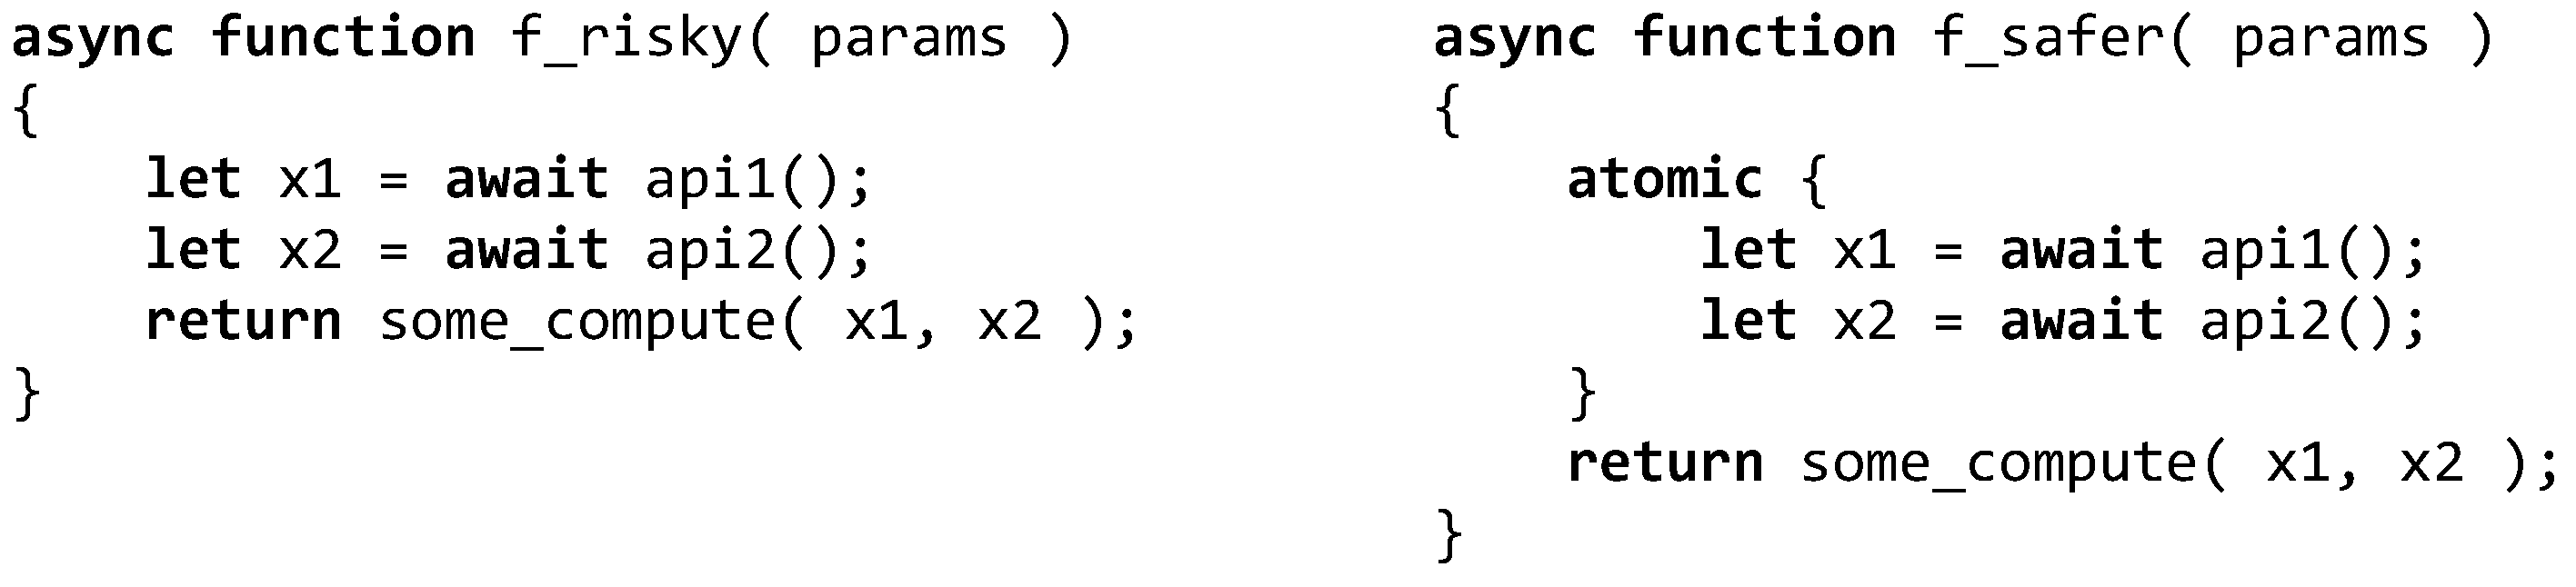
\includegraphics[width=0.9\textwidth]{Code/async_atomic_js}
\caption{A simple sketch of code that could lead to the risky gaps, and a version with an atomic block to eliminate the risk of an atomicity violation.}
\label{fig:async_atomic_js}
\end{figure}

As discussed in the previous section, there are multiple viable strategies for mitigating the risk of atomicity violations created by short-duration chains of continuations.
In this section we explore one of those strategies: adding an atomic block to languages like JavaScript that use event loops, coroutines or similar anonymous multitasking frameworks.
Figure \ref{fig:async_atomic_js} shows a simple sketch of how atomicity violations can arise, and our proposed solution.
Previous research has shown that atomic blocks can be an effective concurrency control mechanism in the multithreading context (for example, \cite{Pankratius2011, Pankratius2014}).
Most importantly for this project, atomic blocks are simpler to use than some alternatives (e.g. explicit mutex locks), and therefore are useful to developers of a wider skill range\footnotemark{}.

\footnotetext{Despite considerable attention from the research community, atomic blocks have not become a common feature in the context of multithreading.
We believe this is primarily due to the substantial implementation challenges and tricky semantic issues with how code in an atomic block should interact with concurrent code that is not in an atomic block.
These issues are not relevant in a cooperative context.}

In this section we show that the combination of anonymous multitasking (e.g. with event loops or coroutines) and atomic blocks is problematic.
We then explore adding a flavor of cooperative threads with atomic blocks to JavaScript.

\subsection{A Definition of Atomic for Event Loops} \label{sec:candidate_atomic}

One reasonalbe definition of atomic in event systems is as follows:

% \cite{Loring2017} Semantics of Asynchronous JavaScript

\begin{enumerate}
\item When some code enters an atomic block, all pending events are removed from the dispatcher and pushed collectively onto a stack of pending events.
\item The code of the atomic block runs as usual, possibly registering new events.
\item When the code reaches the end of the atomic block it pauses to allow events from the dispatcher to run (i.e. the events registered by the atomic block itself).
\item Events are executed as usual (with continuations potentially registering new events).
\item Once the event dispatcher is empty, the code that was waiting at the end of the atomic block can continue; simultaneously the events that were pushed in step 1 are popped and restored to the dispatcher.
\end{enumerate}

Notice that this definition works for nested atomic blocks.
In cases where the body of an atomic block consists of a short linear chain of continuations, this definition would produce exactly the expected effect: the whole chain would run before any concurrent events are processed.
It is when there is branching within the atomic block that the desired semantics get less clear.
Because it is not possible to distinguish between logically continuing the current task and spawning a new one, this definition effectively assumes that all continuations are part of their parent's task, and assumes they should all be contained within the atomic block.

\subsection{Background on Nested Atomics and Spawns}

In this subsection we give a brief review of research on atomic blocks in the context of multithreading and transactional memory.
We will relate this back to event loop systems below.
The tricky semantic issue is how to define thread spawns nested within atomic blocks (and potential further nesting of both).
One good treatment of the formal semantics of this issue is \cite{Moore2008}.
Some of the possibilities that have been explored are:
\begin{itemize}
\item Spawning a thread within an atomic block is an error (static or dynamic) (\emph{spawn-error}).
\item Spawns within atomic blocks are delayed until after the block has completed. (\emph{delay-spawn}).
\item Threads spawned within an atomic block are allowed to run concurrently, and the block is not complete until such threads are finished. (\emph{spawn-contained}).
\item Threads spawned within an atomic block are allowed to run concurrently, and are completely disconnected from the block.
\end{itemize}

Unfortunately, it seems there is no simple definition that works well in all cases.

\emph{Spawn-error} is tempting, since it somehow feels like spawning new tasks is not in the spirit of ``atomic''.
However, this is hard to defend on principle, because there are perfectly reasonable programs that have spawns inside atomic blocks.
More practically, consider a library function that spawns a new task.
\emph{Spawn-error} would make it impossible to wrap a call to such a function in atomic, which can be problematic.
Furthermore, as we will see in the empirical analysis below, programs that seem to have this shape are fairly common.

The \emph{delay-spawn} strategy causes deadlock for code that spawns a thread then waits for it, while still in the atomic block.

The \emph{spawn-contained} strategy causes starvation for code that spawns long-running tasks, because according to this strategy the atomic block is not finished until all spawned tasks are finished.
This is effectively the strategy enforced by the candidate definition of atomic above.

%% A quick example of when the \emph{spawn-contained} policy is problematic:
%% Consider a function that performs a few quick database queries and then sends a potentially slow network request based on the results of the queries.
%% A caller may want to enforce atomicity among the database queries, but wrapping a call to this function in atomic would cause the application to become unresponsive until the network request completed.

\subsection{Do Programs Actually Do this Weird Stuff?}

\begin{table}
  \centering
  \begin{tabular}{|r|r|r|r|r|r|r|}
    \hline
    Limit (ms) &  Total & Linear & Multi L & Multi S & Contain L & Contain S \\
    \hline
    1          &    837 &   66\% &    17\% &   0.7\% &      18\% &     0.2\% \\
    \hline
    10         & 17,885 &   80\% &   4.4\% &   2.1\% &      15\% &     1.3\% \\
    \hline
    100        & 46,515 &   87\% &   3.9\% &   2.3\% &     8.3\% &     1.5\% \\
    \hline
  \end{tabular}
  \caption{XXX subtrees}
  \label{table:subtrees}
\end{table}

Before considering approaches to handing nested atomics and spawning, it is useful to measure whether these patterns occur with any frequency in practice.
If spawning inside atomic blocks is rare, then simple definitions (like \emph{spawn-error}) might be viable.

We analyzed the continuation trees we collected for evidence of spawning within atomic blocks.
Obviously JavaScript lacks both explicit spawning and atomic blocks, so out analysis is inevitably guessing to some extent.
We take continuations with multiple children (i.e. branching) as a suggestion of spawning, and we take multiple related continuations within a small time window as a suggestion of a block that could be atomic.
Specifically, we define \emph{potentially atomic subtrees} (PASs) of a continuation tree to be those that satisfy the following conditions:

\begin{itemize}
\item \emph{Nontrivial}. At least two continuations.
\item \emph{Connected}. Not forests.
\item \emph{Time limited}. The duration from the beginning of the first continuation to the end of the last must be under some time limit.
\item \emph{Maximal}. Proper subtrees of trees that satisfy these conditions do not count.
\item \emph{No Recurring}. Recurring edges are ignored, except for a special case described below.
\end{itemize}

We examined all the PASs in our data set, and found the following shapes.
For some shapes we defined variants of the criteria that we call ``looser'' or ``stricter''.

\begin{itemize}
\item \emph{Linear}. All continuations have at most one child.
  We consider even recurring
\item \emph{Multiple long-lived branches}. Looser version: Has at least two children outside the subtree (can have the same parent).
Stricter version: Has at least two children outside the subtree with different parents.
\item \emph{Contained branch}. Looser version: Has at least one continuation with no children, and at least one continuation with at least one child outside the subtree.
  Stricter version: Same as the loose version, with the additional constraint that there be at least one continuation in the subtree after the one with no children.
\end{itemize}

Table \ref{table:subtrees} shows the total number of PASs and the percentage of each shape for 5 different time limits.
The first thing to observe is that most of the subtrees are linear, but not by an overwhelming margin.
This suggests that a definition of atomic blocks that handled branching poorly could create problems in practice.

A small fraction of the PASs have multiple long-lived branches.
This suggests that the simple candidate definition of atomic given at the beginning of section \ref{sec:candidate_atomic} (\emph{spawn-contained}) would create responsiveness problems.
Implementing any of the other strategies requires that the system have an understanding of which continuations are spawning new tasks versus continuing the current task.

A small fraction of the PASs have contained branches.
This suggests that the \emph{delay-spawn} strategy could create deadlock problems.
Note that even for the stricter version of the contained branch criteria, we cannot say for sure that the longer branch is waiting for the shorter branch.
If it is not waiting, then the \emph{delay-spawn} strategy could be fine.

While further study of more ecosystems and application families is called for, we suggest the following guidelines based on this analysis.
\emph{If} a language designer wants to introduce an atomic block into a cooperatively concurrent system:
\begin{itemize}
\item The system should have explicit task identities.
\item \emph{Delay-spawn} is a good default strategy, because it works fine with long-lived tasks spawned inside atomic blocks and it seems that truly contained spawns that can cause deadlock with this strategy are fairly rare.
\item There should be some mechanism for programmers to override the default for specific atomic blocks and/or specific task spawns.
\end{itemize}

\section{Cooperative Threads and Atomic Blocks for JavaScript}

In this section we discuss the first of our two implementations of cooperative threading with atomic blocks, built on top of generator functions (\texttt{function*}, a.k.a. coroutines).
Atomic blocks have been added to several other languages with preemptive multithreading, at least in an experimental capacity; for example: Haskell \cite{Harris2005}, OCaml \cite{Ringenburg2005}, Java \cite{Herlihy2006}, C/C++ \cite{Ni2008}.
We do not claim any novelty with respect to the basic questions of what atomic blocks should mean.
In fact, it is much easier to implement atomic blocks in the cooperative context.
The main point we explored was how easily this idea can be integrated with popular coding patterns and legacy code.

The core code is in appendix XXX.

We begin by building a flavor of async functions on top of generators; this idea is discussed in the ``Informative Desugaring'' appendix to the official proposal for async functions \cite{Terlson2016}, and has been implemented in several libraries.
The main trick is a stepper process that iteratively calls the \texttt{next} or \texttt{throw} method on the generator until it is done.
The two differences between standard async functions and our variant (which we distinguish by calling \emph{\asyncs{}}) is that ours support an explicit notion of tasks and task spawning, and atomic blocks.

\begin{figure}
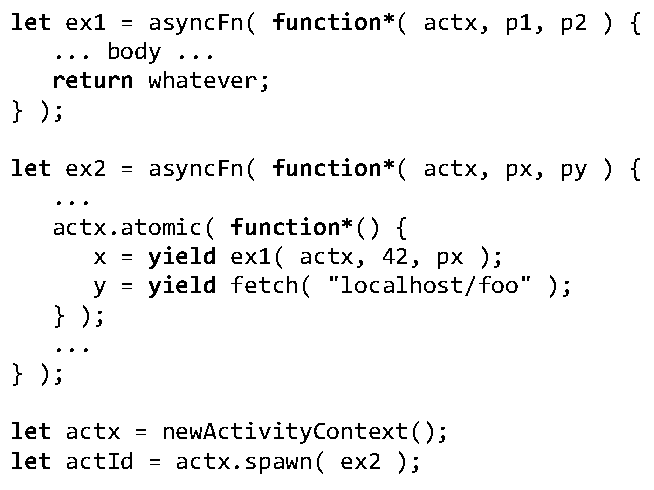
\includegraphics[scale=0.75]{Code/trivial_js}
\caption{A sketch of how the JavaScript library implementation of activities is used.
The syntactic clutter is fairly high because we are using JavaScript function generators (\texttt{function*}) to simulate regular functions in an activities framework.}
\label{fig:trivial_js}
\end{figure}

Implementing explicit tasks requires that when an \asyncs{} function is running it has to ``know'' what task it belongs to.
We explored two solutions to this problem.
The first requires user code to explicitly pass an additional context parameter to all \asyncs{} functions.
This version is nicely explicit, but introduces substantial syntactic overhead.
The second implementation uses a global variable to implicitly pass the task context information to functions that need it.
The stepper process sets this global variable to the correct task context just before taking the next step in each \asyncs{} function.
A third option that we \emph{did not} explore is to use the new metaprogramming facilities in JavaScript to modify definitions of and calls to \asyncs{} functions to explcitly pass a task context parameter.

XXX PARAMS FOR EX2
Figure \ref{fig:trivial_js} gives a tiny example of what our library actually looks like.
XXX

Our \asyncs{} functions mostly integrate well with legacy code.
Any existing Promise-based function can by called, just like in standard async functions (and many callback-based functions can be trivially converted to being Promise-based with the popular \texttt{promisify} library).
Our \asyncs{} functions can be called like regular async functions by legacy code.
However, the legacy code does not know about task contexts, so legacy code calling \asyncs{} functions or other functions provided by our library can result in unexpected results with respect to what task a call ``belongs'' to.
We consider such calls to be unsupported behavior.

We implement atomic by checking in each step of the stepper process whether the current task is blocked.
If it is, it adds itself to a waiting set and blocks until the relevant atomic block ends.
A consequence of this approach is that our library cannot enforce atomicity on chains of continuations registered by legacy code.
This limitation on atomicity-enforcing power is inevitable in a library-based design.
However, if a JavaScript interpreter was to adopt our design natively, it could easily enforce such atomicity in the event dispatcher.

As discussed in the previous section, what makes atomic interesting is how it interacts with task spawns in the body of the atomic.
Without such nesting, atomic could be implemented with a single global variable that stores either the task identity of the task in atomic mode, or an empty token (i.e. \texttt{null}, or whatever).
In order to support a range of options, depending on choices made by user code, our implementation maintains a stack of \emph{atomic contexts}, which is empty when no tasks are in an atomic block.
When a task enters an atomic block, it pushes a new atomic context and saves all currently active tasks as peers in that context.
Those peers will be blocked until that atomic block finishes.


As mentioned previously, there are several reasonable strategies for handling spawns inside atomic.
By default, activities spawned while the program is in atomic mode will be put on hold until the program has exited atomic mode.
This strategy is the default because it is relatively simple, and as long as the atomic block executes relatively quickly (which is how the feature is supposed to be used), the newly spawned activities will experience relatively little delay.
Unlike the multithreading and transactional memory context, where there might be a performance benefit to letting multiple threads simultaneously execute in atomic mode, we are dealing with single-threaded multitasking here.

The only situation in which the \emph{delay-spawn} strategy is problematic is when the code executing the atomic block waits (directly or indirectly) for the newly spawned activity to do something before leaving the atomic block.
In this situation, forcing the new activity to wait could cause the program to deadlock.
For this reason, the spawn function accepts an optional parameter to override the default nesting strategy.
Newly spawned activities can be spawned with the \emph{spawn-contained} strategy.
This allows the newly spawned activity to run, and forces the program to wait at the end of the atomic block for any such activities to complete.

The design that we ended up with is mostly like conventional cooperative multithreading with an atomic block.
In this paper we do not present any formal semantics; rather, we refer to existing work on the semantics of cooperative threads \cite{Abadi2009} and atomic blocks \cite{Moore2008}.
One minor difference we noticed is that there is an implicit interruption point (i.e. yield) at the end of every step of the stepper process.
Looking at this slightly differently, it can be seen as an implicit yield just before and after each call to an \asyncs{} function.
While these implicit yields arose as a side-effect of our libraries implementation, upon further analysis, this design seems interesting in its own right.
We named these cooperative threads with implicit yields before and after non-atomic calls \emph{activities}, and we analyze their pros and cons in the next section.

We briefly note an efficiency opportunity enabled by atomic blocks.
For short chains of continuations, the overhead associated with moving in and out of the event dispatcher can be nontrivial.
In a version of JavaScript with native atomic blocks, it would be possible for a just-in-time compiler to fuse atomic chains of continuations into a single function, eliminating this overhead.

% XXX Doppio ??? \cite{Vilk2014}

\section{An Atomic Block for C (Design)}

In the previous section, we looked at what we called \emph{activities} (cooperative threads, with implicit yields around calls and an atomic block) in the context of a JavaScript library.
In this section and the next we look at adding the same language feature as an extension to C that we call \charcoal{}.
There are two questions this lets us investigate:
What, if any, language design issues does this feature create in a more ``native'' context?
Can this feature be implemented efficiently in a context where basic overheads for things like function calls are very low?

Like the JavaScript version, the primary additions are spawn (which we call \texttt{activate}) and \texttt{atomic} primitives.
We also needed to add a \texttt{yield} primitive, since this does not exist in standard C.

To illustrate our design, we use an example stolen from \cite{Krohn2007}; a standard C version is in Figure \ref{fig:charcoal_multidns_seq}.
This example performs \texttt{N} DNS lookups using the standard \texttt{getaddrinfo} procedure.

The \charcoal{} version in Figure \ref{fig:charcoal_multidns_sem} performs these lookups concurrently.
It has a parameter (\texttt{max\_conc}) to limit the number of DNS requests that will be sent concurrently to avoid flooding the network with too many requests.

We add some syntactic convenience to the plain spawn to get the \emph{activate} statement (see line 10 of Figure \ref{fig:charcoal_multidns_sem}).
The body of the activate statement runs concurrently (but \emph{not} in parallel) with the statement's continuation.

\begin{figure}
    \centering
    \begin{minipage}[t]{0.47\textwidth}
        \centering
        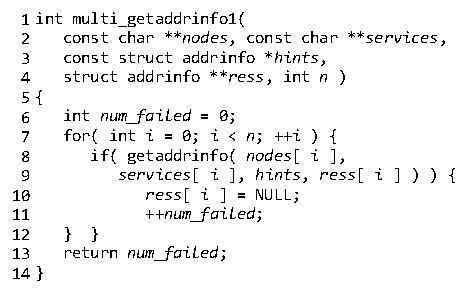
\includegraphics[width=1.0\textwidth]{Code/multi_getaddrinfo_seq}
        \caption{This is a plain C version of the DNS fetcher example.
  This version is entirely \emph{sequential}.}
        \label{fig:charcoal_multidns_seq}
    \end{minipage}\hfill
    \begin{minipage}[t]{0.47\textwidth}
        \centering
        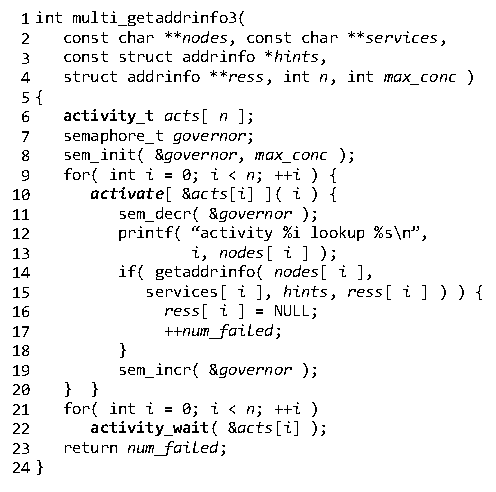
\includegraphics[width=1.0\textwidth]{Code/multi_getaddrinfo_sem}
        \caption{This is a \charcoal{} version of the DNS fetcher that can fetch multiple entries concurrently.
          This version of the DNS fetcher limits the number of concurrent requests to \texttt{max\_conc}.}
        \label{fig:charcoal_multidns_sem}
    \end{minipage}
\end{figure}

The activate statement takes as a parameter a pointer to application-allocated memory for storing activity metadata.
In the example, the memory for storing activity information is allocated locally.
Because of this the example procedure must wait for all the activities it spawns to finish.
(Returning before they finish could cause the program to access deallocated memory).
It would be possible to change the interface so that the caller passes in the backing memory, or to use dynamic allocation and leave the deallocation to the caller.
In either of these cases, the procedure could return while the activities were still fetching DNS information, allowing the application to go on with other work.

\subsection{Yield Insertion}

Unlike the JavaScript library implementation, where interruption points before and after calls happen naturally, the \charcoal{} implementation has to insert yields during compilation.

This rule helps ensure responsiveness by default.

In the example code above, the system will automatically insert four yields: one each before and after the two calls.
Without further information, it should be assumed that the called functions themselves have more yields in their implementations.

XXX C code sequence points

XXX refactoring issue


There are two ways a program can still become unresponsive.
The first is by wrapping a long-running part of the program in atomic.
The second is long-running loops with no calls (or explicit yields) in their body.
Both of these should be considered concurrency bugs to be managed with the usual software reliability tools (testing, code review, verification, etc).


Automatic yield insertion makes activities more like preemptive threads than conventional cooperative threads.
However, activities are still more resistant to concurrency bugs than threads by default, because the granularity of scheduling is coarser.
Between calls and explicit yield invocations, code is guaranteed to execute atomically.
For example, classic data races are impossible with activities.


\subsection{Shared Variables}

The parentheses after the \texttt{activate} keyword are for controlling whether local variables are captured by-value or by-reference.
The default is by-reference, which is how most of the variables are used in this example.
This means that all the activities read and write a shared instance of that variable.
The exception is \texttt{i} which is used as a name of sorts in the \texttt{printf} call.
Each activity gets its own copy of \texttt{i}, whose initial value is whatever the variable's value was at activity creation time.
If there were a modification to \texttt{i} inside \texttt{activate}, each activity would be modifying its own copy.

\subsection{Atomic}
\label{sec:atomic}

Any statement, expression or procedure declaration/definition in \charcoal{} can be ``wrapped'' with atomic.
In the dynamic scope of an atomic block, the current activity cannot be interrupted.
In other words, any yields that would have happened are overridden/suppressed by atomic.

In the example, the compiler will insert yields before and after the calls to \texttt{printf} and \texttt{getaddrinfo}.
If the programmer wanted to suppress some of these yields, they could use \atomic{}.
For example, it would be reasonable to wrap the \texttt{printf} call in \atomic{}, since it will complete quickly (relative to \texttt{getaddrinfo}), and there is little to be gained by switching to another task at that point.
Wrapping the \texttt{getaddrinfo} call in atomic would be a performance bug, because that would force the DNS lookups to be executed sequentially.

\section{An Atomic Block for C (Implementation)}

There are a few interesting features of our implementation of activities in the context of \charcoal{}, which we describe in this section: the allocation of call frames, the implementation of the yield primitive, and compiling a version of each procedure for yielding and atomic mode.

\subsection{Call Frame Allocation}

Procedure call frame allocation strategies are important for any thread-like abstraction.
The first few sections below review the most widely used strategies.
Then we describe a new approach that we call \emph{hot stacking}.

\subsubsection{Contiguous Allocation}

A common and simple strategy is to pre-allocate a moderately large block of memory for each thread.
Individual frames are allocated contiguously within this area.
This strategy leads to the fastest calling and returning.
However, it has two memory inefficiencies: (1) many frameworks and applications conservatively allocate more memory than is necessary; (2) in many implementations the minimum block size is page, which is too big for very ``small'' threads.
Also, if a mistake of some sort leads to under-allocation for a thread's block, a variety of nasty failures can happen.

\subsubsection{Individual Heap Allocation}

At the other extreme of the time/memory efficiency spectrum, systems can individually allocate each frame, linking them together with pointers.
This avoids the memory concerns associated with contiguous allocation.
However, heap allocation of frames comes at a time cost for calls and returns.

Simple implementations of heap allocation can be more than an order of magnitude slower than contiguous allocation.
More sophisticated implementations can be substantially more efficient (e.g. \cite{Shao2000}).
However, even the most efficient implementations that we are aware of are still slower than contiguous allocation for call-heavy code.

\subsubsection{Split/Segmented Stacks}

Some languages have experimented with a hybrid strategy called \emph{split}, \emph{segmented}, or \emph{linked} stacks.
The idea is that space is allocated in small segments or chunks.
In the common case, frames are allocated contiguously within the top segment.
When a thread reaches the end of its segment it allocates a new one and links it to the previous one with pointers.
This idea has been appealing to several language implementers; as fairly recent examples, early implementations of Rust and Go both used it.
Unfortunately it has unpleasant \emph{uncommon} case behavior called \emph{stack thrashing} or the \emph{hot split} problem.
When there are frequent calls/returns right at the boundary between segments, the overhead can be quite high.
The implementers of Rust \cite{Anderson2013} and Go \cite{Anastasopoulos2014} both abandoned this strategy in later versions.

% Also \cite{Middha2008}

\subsubsection{Growable/Copying Stacks}

Since version 1.3, the Go language has used an unusual allocation strategy, where each goroutine starts with a relatively small continguous block of memory that is resized when necessary \cite{Cheney2014, Morsing2014}.
Resizing the block in-place is obviously desirable from a performance perspective, but if the address range the block would be resized into is not free, then it must be relocated instead.
This is only possible because the Go language implementation keeps track of all pointers to procedure local memory and can update them during relocation.
Clearly this would not work for languages like C and C++ that expose raw pointers to application code.
Similarly to the hot split problem, this strategy suffers from pauses when the stack has to be relocated.
In practice these pauses are rare, but they are unpredictable and can be expensive.

\subsubsection{Hot Stacking}

The call frame allocation strategy introduced in this paper is a hybrid of contiguous and individual heap allocation.
The key observation is that the speed of frame allocation is only important for \emph{short-lived calls}.
For \emph{long-lived calls}, the overhead of the call and return operations is unimportant, because it can be amortized over the long running time of the call.
So the main idea of hot stacking is that long-lived frames are individually allocated and (most) short-lived frames are contiguously allocated in memory that is shared among tasks.

When a new task is created, its initial frame is individually allocated.
When it makes a call, the implementation decides which kind of allocation to do for that call.
If the system expects the call to be long-lived, it should allocate its frame individually in the heap.
If the system expects the call to be short-lived, it should acquire a large block of memory and start allocating contiguously in that block.
All subsequent calls made by that task will use contiguous allocation until the call that triggered the mode switch returns, at which point the task will go back to individual allocation.
During the time that a task is allocating contiguously, no other task can use that task's block of memory.

For this strategy to be efficient, the implementation has to know when it should switch from individual allocation to contiguous allocation (or at least be ``right'' most of the time).
If it switches ``too late'', then short-lived frames will be allocated individually, causing some time overhead.
If it switches ``too early'', then long-lived frames will be allocated in a large block, preventing other tasks from using that block.
The former problem is clearly the less disruptive of the two, but they should both be considered performance bugs.
If the implementation gets this Goldilocks problem right, then most frame allocations will be performed contiguously, but the large blocks will never be locked down by a task for a very long time.

\emph{Atomic blocks} are one tool an implementation could use to choose when to switch allocation modes.
That is, all calls made in atomic mode use contiguous allocation, and all calls made in interruptible mode use individual allocation.
This approach has a couple important benefits:
\begin{itemize}
\item It is very simple; the implementation does no analysis or inference.
\item It is under programmer control; programmers can widen or narrow the scope of atomic blocks, if they are dissatisfied with how the allocation is done in specific contexts.
\end{itemize}

Languages that do not have atomic blocks could conceivably use hot stacking, but the implementation would have to be more sophisticated.
We are unsure if this is a promising idea, and leave investigation of it to future work.

In the microbenchmarking section below we provide evidence that this strategy captures the benefits of individual allocation (per-task memory overhead is small) and contiguous allocation (calls and returns are fast when it matters).

In languages with cooperative threads that disallow nested spawns, the implementation of hot stacking can be especially simple.
In this case, a whole program only ever needs a single large block of memory for contiguous allocation.
If nested spawns are allowed, then we have to consider the possibility of two tasks running concurrently, both in atomic mode.
While we expect this scenario to be quite rare in practice, it is possible, so our implementation has to be prepared for it.
We do this by dynamically allocating additional large blocks as necessary.
By default, our implementation keeps exactly one large block allocated as long as at most one task is in atomic mode.

Other than the nested spawn issue, we believe hot stacking to be free of the kinds of uncommon case performance problems that the segmented and growable stacks strategies have.

The name \emph{hot stacking} is a reference to the practice called \emph{hot racking} or \emph{hot desking}, where some limited resource (e.g. a bunk or desk) is used in shifts by multiple people.
In our case, the resource is the memory blocks for contiguous frame allocation, and they are shared by multiple tasks.
The word \emph{hot} is also a reference to the fact that this top of stack area should remain hot in the memory hierarchy/cache sense as long as any code is running, because all tasks use the same block of memory for their short-lived calls.
We speculate that this cache effect could give hot stacking a small performance advantage over strategies where tasks do not share stack memory at all, but we have not attempted to measure this effect yet.

%% Soemthing in here is kinda related to ideas from the Cilk-5 implementation \cite{Frigo1998}.

\subsection{Yield Implementation}
\label{sec:yield_imp}

Automatic yield insertion makes frequent yielding common, which makes the efficiency of yielding important.
We explored three yield implementation ideas:

\begin{itemize}
\item Zero overhead yields in atomic mode
\item Infrequent context switching
\item Fast non-switching yield
\end{itemize}

\subsubsection{Yield in Atomic Mode}

There are important differences at the implementation level between how code executes in yielding versus atomic mode, not least among them the call frame allocation strategy.
To implement this dual mode concept in a reasonably simple and efficient way, the current \charcoal{} implementation generates two versions of each procedure: one for each mode.
The yielding mode implementation includes inserted yields and assumes its own frame was individually allocated.
The atomic mode implementation does not include yields, which effectively means that yields in atomic mode are zero-overhead.

This implementation strategy could lead to a substantial increase in code size (more than 2$\times$).
We believe this problem can be managed, based on the assumption that in practice most procedures are called only in either interruptible or atomic mode, not both.
This means that an implementation could either rely on a smart linker to perform dead code elimination, or start with a single version and use runtime optimization to generate the other one on-demand.

\subsubsection{Actual Yields}

The most important factor in the implementation of the yield primitive is that most yield invocations should not result in context switching, even if other activities are ready to run.
In well designed activity code, the time between yield invocations should be in the range of microseconds to milliseconds.
Context switching has the moderate direct cost of manipulating a handful of data structures in the runtime system, and the potentially higher indirect cost of cache thrashing.
Therefore in the common case, most yields should return control to the running task.
Actual context switches should happen a relatively low frequency, perhaps every few milliseconds.

As described in the previous section, code that is compiled in atomic mode does not have yields at all, so yield performance is not an issue for the most performance critical loops.
However, we expect that moderately frequent yielding (perhaps as frequently as many per microsecond) would be common in practice.
Therefore, the performance of the yield primitive does matter.

The simplest implementation of yield would check a counter or clock of some sort.
Reasonably efficient implementations of this strategy would certainly be non-portable (e.g. using processor-specific counter registers) and probably still be somewhat expensive.
Instead the current \charcoal{} implementation uses a periodic system timer/alarm that delivers a signal to the program, as long as there is at least one runnable activity waiting.
The handler for this signal atomically modifies a global variable.
The yield primitive atomically reads this global variable; as long as it has not changed control returns to the running task.
Therefore, in the common case, the cost of a yield is an atomic read and a (highly predictable) branch, plus a fast call and return to get to the yield code itself.
(Of course the yield code can be inlined, but that is \emph{not} obviously a good idea because inlining functions with many call sites can pollute the instruction cache and branch predictor.)

\subsubsection{Function Pointers}

One challenge with a dual implementation strategy is how to handle function pointers.
When the address of a function is taken it is not possible, \emph{in general}, to know which mode the function will eventually be called in.
The current implementation generates a small piece of code for every function that can be called in either yielding or atomic mode.
It accepts an additional implicit parameter, which controls which actual version gets called.
This makes indirect calls somewhat more expensive than in plain C.
However, indirect calls are already expensive enough that there is an extensive body of research on how to convert them to direct calls (e.g. \cite{Dean1995}), so adding a modest amount of overhead to indirect calls should not have a large performance impact on most applications.

\subsection{System Calls}

One of the benefits commonly associated with light-weight multitasking primitives is cheap and responsive system interaction via non-blocking I/O interfaces, like epoll, kqueue and I/O Completion Ports.
The current \charcoal{} implementation uses \texttt{libuv} to handle this part.
At startup, the runtime system spawns a thread that runs a \texttt{libuv} event loop.
The \charcoal{} implementation includes implementations of standard C functions that translate blocking calls into sending a message to the I/O thread and suspending the current activity.
When the event completes, the system makes the relevant activity runnable again.

This architecture works, but it adds overhead for fast system calls that would be better implemented without any inter-thread communication.
We speculate that integrating the event processing with application code in the same thread could remove some performance overhead.
The \texttt{libuv} maintainers have discussed this as a ``pull'', versus the current ``push'' architecture, which they may implement in a future version \cite{libuv2014}.
% XXX yield checks for event loop changes

\subsection{Translation}

We use a modified version of Cil \cite{Necula2002} to translate \charcoal{} to plain C with calls to our runtime system, which is written in C.

\section{Microbenchmarking Activities in C}

To investigate the performance of activities, we wrote microbenchmarks with the \charcoal{} implementation.
All tests were run on a machine with the specs listed in Table \ref{table:specs}.
Depending on the benchmark, we compare the \charcoal{} implementation against plain C, C compiled with gcc's split stack implementation, Go or C plus the default Linux threads implementation.
All speed-related tests were compiled at optimization level \texttt{-O2}.
For speed-related tests we ran the benchmark 5 times and report the fastest result.

\begin{table}
  \centering
  \begin{tabular}{|l|l|}
    \hline
    OS & Ubuntu Linux 14.04 \\
    \hline
    Kernel & 3.13.0-68-generic \\
    \hline
    Processor & 4 GHz Intel Core i7 \\
    \hline
    Memory & 8 GB 1600 MHz DDR3 \\
    \hline
    Compiler & gcc 4.8.4 \\
    \hline
    Go & 1.5.3 \\
    \hline
  \end{tabular}
  \caption{Specs of the test system}
  \label{table:specs}
\end{table}

\subsection{Memory Overhead}

Like coroutines (e.g. in their modern C++ incarnation), activities have very low memory overhead; approximately whatever is needed to store a dozen pointers.
It is interesting to compare this with goroutines.
The Go implementation uses a sophisticated stack growing process to avoid pre-allocating a large amount of memory for call frames.
However, the minimum size is still relatively large (in the neighborhood of a kilobyte), more than a factor of 6 greater than activities in \charcoal{}.

\subsection{Task Spawn and Switching Speed}

Unsurprisingly, activities are dramatically faster than system threads when it comes to spawning and switching between tasks.
The speed difference is over an order of magnitude, as measured by microbenchmarks.
The primary difference here is that threads must make system calls to do these things, whereas with activities they can be done entirely in user mode.

In these benchmarks, Go was slightly faster than \charcoal{}.
We expect this is because the Go team has put a lot of engineering effort into optimizing these concurrency primitives.
We see no reason that the \charcoal{} implementation could not be optimized just as well.

The speed of these primitives have a big impact on the practical minimum granularity of tasks.
In both \charcoal{} and Go that overhead is closer to that of a method call than the equivalent thread operations.
That means that multitasking can be used in interesting ways in those languages that they cannot with threads.

\subsection{Just Calling}

Our next microbenchmark measures the overhead of hot stacking.
This test is a simple recursive function that calls itself twice and performs a very small computation at the ``leaves''; the code is in Figure \ref{fig:micro_calling}.

\vspace{1em}
\begin{tabular}{|l|r|r|r|}
  \hline
   & user & sys & wall \\
  \hline
  \hline
  Plain C & 0.77 & 0.00 & 0.77 \\
  \hline
  Individual Allocation & 42.4 & 0.04 & 42.6 \\
  \hline
\end{tabular}
\vspace{1em}

These numbers are in nanoseconds per call/return.
This difference is nearly two orders of magnitude, which is painful for \charcoal{}.
However, there are three caveats to keep in mind.
First, the \charcoal{} implementation is not highly optimized; the allocator used in this test was the default system malloc.
Surely a more tuned implementation would close the gap to some extent.
Second, this is a microbenchmark; no application spends all of its time just calling and returning, so these numbers are a fairly high upper bound on the real application performance impact of calling overhead.

\begin{figure}
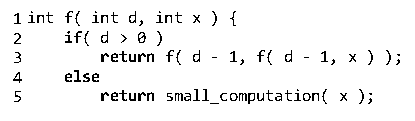
\includegraphics{Code/just_calling_benchmark}
\caption{The microbenchmark for measuring call frame allocation overhead.}
\label{fig:micro_calling}
\end{figure}

Most importantly, all the calls in the first version of this test were performed in yielding mode.
In atomic mode, calls and returns in \charcoal{} are just as efficient as plain C.
In well-tuned \charcoal{} code, most of the leaf and near-leaf calls should be performed in atomic mode.
To simulate this effect, we modified the benchmark to the version in Figure \ref{fig:micro_calling_n}.
The parameter \texttt{N} controls how deep in the call tree the benchmark uses yielding mode, before switching to atomic.

\vspace{1em}
\begin{tabular}{|l|r|r|r|}
  \hline
   & user & sys & wall \\
  \hline
  \hline
  Plain C & 0.77 & 0.00 & 0.77 \\
  \hline
  gcc split stacks\footnotemark{} & 1.00 & 0.15 & 1.15 \\
  \hline
  Go & 2.80 & 0.20 & 3.00 \\
  \hline
  Hot Stacking, \texttt{N} = 4 & 11.00 & 0.01 & 11.00 \\
  \hline
  Hot Stacking, \texttt{N} = 8 & 1.54 & 0.00 & 1.55 \\
  \hline
\end{tabular}
\vspace{1em}

\footnotetext{This benchmark does not create stacks deep enough to exceed the default size of a single segment of gcc's split stack.
So we modified the benchmark for the split stack case to make a linear chain of calls instead of a binary tree.}

This shows that with a modest fraction of the (static) calls performed in atomic mode, the calling overhead gets down to less than a factor of 2.
Combined with the observations above about tuning the language implementation, we believe this overhead would be barely noticeable for most applications.
Also it is worth noting that this is the price to be paid for the extremely low memory overhead of activities.

Hot stacking with \texttt{N} = 8 outperforms Go on this benchmark by a modest margin.
It is interesting that the gap between plain C and Go is as large as it is, given the Go implementation team's famous focus on low-level performance details.

gcc's split stack implementation outperforms hot stacking by a small margin on this benchmark.
However, as noted previously split stacks have bad performance in the pathological case where calls are made at high frequency right at the edge of a segment.

\begin{figure}
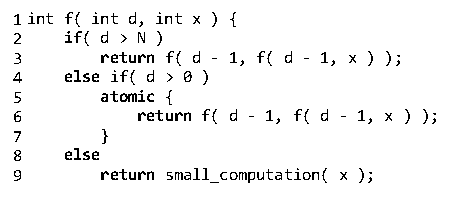
\includegraphics{Code/just_calling_n_benchmark}
\caption{The call/return microbenchmark modified to make some calls in atomic mode.}
\label{fig:micro_calling_n}
\end{figure}

\subsection{Yielding}

As described in section \ref{sec:yield_imp}, yield frequency can be managed fairly easily and the yield primitive is designed to have a very fast common path.
Nevertheless, it is important to minimize yielding in loops.

To quantify yielding overhead, we benchmarked a simple but problematic function from the C standard library: \texttt{strcmp}.
\texttt{strcmp} is tricky for a few reasons:
First, the input strings can be arbitrarily long, so never yielding could cause unresponsiveness.
Second, the body of the loop is extremely simple; good implementations are just a few assembly instructions.
This means that yielding every iteration causes significant performance overhead.
Third, the continued execution of the loop depends on the data read in each iteration, so loop tiling/blocking tricks do not work.
The best-performing implementation we have found so far appears in Figure \ref{fig:strcmp}.

\begin{figure}[htp]
\includegraphics[left]{Code/plain_strcmp}%
  \\
\includegraphics[left]{Code/strcmp_benchmark}%
\caption{Two implementations of \texttt{strcmp}.
  Top is a plain C version.
  Bottom is a \charcoal{} implementation aimed at minimizing yield overhead.}

\label{fig:strcmp}

\end{figure}


%% \begin{figure}
%%     \centering
%%     \begin{subfigure}[b]{0.3\textwidth}
%%         \hspace{-1.5cm}
%%         \includegraphics{plain_strcmp}
%%         \caption{}
%%     \end{subfigure}
%%     ~ %add desired spacing between images, e. g. ~, \quad, \qquad, \hfill etc. 
%%       %(or a blank line to force the subfigure onto a new line)
%%     \begin{subfigure}[b]{0.3\textwidth}
%%         \hspace{-1.5cm}
%%         \includegraphics{strcmp_benchmark}
%%         \caption{}
%%     \end{subfigure}
%%     \caption{Two implementations of \texttt{strcmp}.
%%       (a) is a plain C version.
%%       (b) is a \charcoal{} implementation aimed at minimizing yield overhead. }
%%     \label{fig:strcmp}
%% \end{figure}

In the code \texttt{YIELD\_FREQ} controls how frequently the loop yields.
The effect is that once every $2^{\mathtt{YIELD\_FREQ}}$ iterations there is a yield.

\vspace{1em}
\begin{tabular}{|l|r|}
  \hline
  Plain C & 430 \\
  \hline
  \charcoal, \texttt{YIELD\_FREQ = 4} & 1070 \\
  \hline
  \charcoal, \texttt{YIELD\_FREQ = 8} & 519 \\
  \hline
  \charcoal, \texttt{YIELD\_FREQ = 12} & 446 \\
  \hline
\end{tabular}
\vspace{1em}

These numbers are in microseconds per \texttt{strcmp} of two identical strings of 1MB length.
These data show that yielding is not free, but with a little careful tuning the yield overhead can be brought quite low.

When the inputs to \texttt{strcmp} are known to be short, the caller can wrap the call in atomic.
The atomic version should perform identically to the plain C implementation.

% \subsection{Code Size}

\subsection{Microbenchmark Summary}

Like all well implemented coroutines, the \charcoal{} implementation has extremely low memory and time overhead for basic concurrency primitives.
Hot stacking and frequent yielding are potential performance issues, but our tests indicate that at these overheads can be managed.

Though we do not have experience with writing large programs in \charcoal{} yet, we expect that relatively little code will require the kinds of contortions shown in the \texttt{strcmp} example.
Moreover, almost all such code will be in tight inner loops in library code.
This is exactly where writing somewhat weird code for performance reasons is acceptable.

%% \section{Foreign Code}

%% Foreign code (including legacy code) will never yield.  This could lead
%% to starvation pretty easily.  Here are three strategies:

%% \begin{itemize}
%% \item Do nothing.
%%   Just run the foreign code.
%%   This is a perfectly reasonable strategy as long as the foreign code does not run for a long time.
%% \item Run the foreign code in its own thread.
%%   If it has not returned by the end of some time slice, pause it to allow other activities to run.
%%   This runs the risk of creating atomicity violations galore.
%%   It also reintroduces the possibility of data races.
%%   However, it might be a reasonable strategy in situations where there is very little sharing between the foreign code and the rest of the application.
%% \item Run the foreign code in its own thread, but only interrupt it at special ``safe-ish'' points, like system calls.
%%   This is a compromise between the previous two strategies in the sense that it opens the door to both starvation and atomicity violations, but provides some (imperfect) protection against both.
%% \end{itemize}

%% We have not thought at all about what the best default is or what syntactic sugar would be nice.

%% Another important implementation issue to consider is foreign code that calls back in to activity-aware code.
%% There will definitely be some fancy footwork necessary there, no matter which strategy is used.

\section{Related Work}

Our activities are clearly closely related to many flavors of cooperative threads.
Most commonly, cooperative threads rely on programs explicitly invoking yield to permit task switching.
Boudol proposes a slightly different approach to automatic yield insertion in cooperative threads \cite{Boudol2007}.
We believe that automatically inserting yields before and after calls by default creates a more predictable environment for programmers.

The other major difference is the atomic block, which this paper shows is not a trivial addition to a language.
We are not aware of any other research on the combination of cooperative threads and atomic blocks.

One weakness that activities share with most multitasking frameworks is that activities cannot easily be run in parallel.
The authors are not optimistic about running cooperative threads in parallel, but there are researchers pursuing this idea \cite{ONeill2015, Boussinot2006, Dabrowski2006}.


%% Threads are the only multitasking abstractions discussed in this paper that naturally allow the parallel execution of tasks.
%% The authors view this as closer to a bug than a feature.
%% Serial multitasking abstractions like events and coroutines (and activities) can be used in combination with parallelism frameworks like processes and threads.
%% The authors consider providing both parallelism and multitasking in a single language features (like threads) mostly a bad idea.
%% Nevertheless, in the discussion section at the end of this paper we speculate about the feasibility of running activities in parallel.


% Threads without the Pain

%% \textbf{Hybrids}.
%% Researchers have long understood the weaknesses of existing multitasking abstractions.
%% Many proposals have been made for event/thread hybrids; for example: \cite{Boudol2007, Boussinot2006, Cunningham2005, Dabrowski2006, Fischer2007, Kerneis2014, Krohn2007, Li2007, Behren2003}.
%% A detailed comparison with all of these proposals is beyond the scope of this paper.
%% In the related work section we highlight the differences with the ones that are most similar to ours.


\section{Summary and Discussion}

In this paper we presented evidence that web applications seem to be highly exposed to atomicity violations.
We note that adding an atomic block would help programmers avoid these problems, and discussed how that addition can be achieved.
Perhaps the most important slogan to take from this paper is that the atomic versus async decision should be made by callers, not implementers of APIs.
We showed that our design can be implemented efficiently in a dialect of C.
We believe that our design combines the benefits of existing cooperative concurrency frameworks in a new and interesting way.


%% Acknowledgments
%% \begin{acks}                            %% acks environment is optional
%%                                         %% contents suppressed with 'anonymous'
%%   %% Commands \grantsponsor{<sponsorID>}{<name>}{<url>} and
%%   %% \grantnum[<url>]{<sponsorID>}{<number>} should be used to
%%   %% acknowledge financial support and will be used by metadata
%%   %% extraction tools.
%%   This material is based upon work supported by the
%%   \grantsponsor{GS100000001}{National Science
%%     Foundation}{http://dx.doi.org/10.13039/100000001} under Grant
%%   No.~\grantnum{GS100000001}{nnnnnnn} and Grant
%%   No.~\grantnum{GS100000001}{mmmmmmm}.  Any opinions, findings, and
%%   conclusions or recommendations expressed in this material are those
%%   of the author and do not necessarily reflect the views of the
%%   National Science Foundation.
%% \end{acks}




% We recommend abbrvnat bibliography style.

% \bibliographystyle{abbrvnat}
% \bibliographystyle{abbrv}

% The bibliography should be embedded for final submission.

\bibliography{./charcoal.bib}

%% \begin{thebibliography}{../../../../Documents/PapersForReferencing/biy_all_research.bib}
%% \softraggedright

%% \end{thebibliography}

\end{document}
